%% bare_conf.tex
%% V1.3
%% 2007/01/11
%% by Michael Shell
%% See:
%% http://www.michaelshell.org/
%% for current contact information.
%%
%% This is a skeleton file demonstrating the use of IEEEtran.cls
%% (requires IEEEtran.cls version 1.7 or later) with an IEEE conference paper.
%%
%% Support sites:
%% http://www.michaelshell.org/tex/ieeetran/
%% http://www.ctan.org/tex-archive/macros/latex/contrib/IEEEtran/
%% and
%% http://www.ieee.org/

%%*************************************************************************
%% Legal Notice:
%% This code is offered as-is without any warranty either expressed or
%% implied; without even the implied warranty of MERCHANTABILITY or
%% FITNESS FOR A PARTICULAR PURPOSE! 
%% User assumes all risk.
%% In no event shall IEEE or any contributor to this code be liable for
%% any damages or losses, including, but not limited to, incidental,
%% consequential, or any other damages, resulting from the use or misuse
%% of any information contained here.
%%
%% All comments are the opinions of their respective authors and are not
%% necessarily endorsed by the IEEE.
%%
%% This work is distributed under the LaTeX Project Public License (LPPL)
%% ( http://www.latex-project.org/ ) version 1.3, and may be freely used,
%% distributed and modified. A copy of the LPPL, version 1.3, is included
%% in the base LaTeX documentation of all distributions of LaTeX released
%% 2003/12/01 or later.
%% Retain all contribution notices and credits.
%% ** Modified files should be clearly indicated as such, including  **
%% ** renaming them and changing author support contact information. **
%%
%% File list of work: IEEEtran.cls, IEEEtran_HOWTO.pdf, bare_adv.tex,
%%                    bare_conf.tex, bare_jrnl.tex, bare_jrnl_compsoc.tex
%%*************************************************************************

% *** Authors should verify (and, if needed, correct) their LaTeX system  ***
% *** with the testflow diagnostic prior to trusting their LaTeX platform ***
% *** with production work. IEEE's font choices can trigger bugs that do  ***
% *** not appear when using other class files.                            ***
% The testflow support page is at:
% http://www.michaelshell.org/tex/testflow/



% Note that the a4paper option is mainly intended so that authors in
% countries using A4 can easily print to A4 and see how their papers will
% look in print - the typesetting of the document will not typically be
% affected with changes in paper size (but the bottom and side margins will).
% Use the testflow package mentioned above to verify correct handling of
% both paper sizes by the user's LaTeX system.
%
% Also note that the "draftcls" or "draftclsnofoot", not "draft", option
% should be used if it is desired that the figures are to be displayed in
% draft mode.
%
\documentclass[10pt,conference,compsocconf]{IEEEtran}
\usepackage{times}
\usepackage[utf8]{inputenc}
\usepackage[ngerman]{babel}
\usepackage[babel,german=quotes]{csquotes} % Für gute Anführungszeichen
\usepackage{float}
\usepackage{listings}
\usepackage{tabu}

\usepackage{caption}
\captionsetup{font=footnotesize,justification=centering,labelsep=period}


% Some very useful LaTeX packages include:
% (uncomment the ones you want to load)


% *** MISC UTILITY PACKAGES ***
%
%\usepackage{ifpdf}
% Heiko Oberdiek's ifpdf.sty is very useful if you need conditional
% compilation based on whether the output is pdf or dvi.
% usage:
% \ifpdf
%   % pdf code
% \else
%   % dvi code
% \fi
% The latest version of ifpdf.sty can be obtained from:
% http://www.ctan.org/tex-archive/macros/latex/contrib/oberdiek/
% Also, note that IEEEtran.cls V1.7 and later provides a builtin
% \ifCLASSINFOpdf conditional that works the same way.
% When switching from latex to pdflatex and vice-versa, the compiler may
% have to be run twice to clear warning/error messages.


% *** CITATION PACKAGES ***
%
%\usepackage{cite}
% cite.sty was written by Donald Arseneau
% V1.6 and later of IEEEtran pre-defines the format of the cite.sty package
% \cite{} output to follow that of IEEE. Loading the cite package will
% result in citation numbers being automatically sorted and properly
% "compressed/ranged". e.g., [1], [9], [2], [7], [5], [6] without using
% cite.sty will become [1], [2], [5]--[7], [9] using cite.sty. cite.sty's
% \cite will automatically add leading space, if needed. Use cite.sty's
% noadjust option (cite.sty V3.8 and later) if you want to turn this off.
% cite.sty is already installed on most LaTeX systems. Be sure and use
% version 4.0 (2003-05-27) and later if using hyperref.sty. cite.sty does
% not currently provide for hyperlinked citations.
% The latest version can be obtained at:
% http://www.ctan.org/tex-archive/macros/latex/contrib/cite/
% The documentation is contained in the cite.sty file itself.


% *** GRAPHICS RELATED PACKAGES ***
%
\ifCLASSINFOpdf
\usepackage[pdftex]{graphicx}
% declare the path(s) where your graphic files are
% \graphicspath{{../pdf/}{../jpeg/}}
% and their extensions so you won't have to specify these with
% every instance of \includegraphics
% \DeclareGraphicsExtensions{.pdf,.jpeg,.png}
\else
% or other class option (dvipsone, dvipdf, if not using dvips). graphicx
% will default to the driver specified in the system graphics.cfg if no
% driver is specified.
% \usepackage[dvips]{graphicx}
% declare the path(s) where your graphic files are
% \graphicspath{{../eps/}}
% and their extensions so you won't have to specify these with
% every instance of \includegraphics
% \DeclareGraphicsExtensions{.eps}
\fi
% graphicx was written by David Carlisle and Sebastian Rahtz. It is
% required if you want graphics, photos, etc. graphicx.sty is already
% installed on most LaTeX systems. The latest version and documentation can
% be obtained at: 
% http://www.ctan.org/tex-archive/macros/latex/required/graphics/
% Another good source of documentation is "Using Imported Graphics in
% LaTeX2e" by Keith Reckdahl which can be found as epslatex.ps or
% epslatex.pdf at: http://www.ctan.org/tex-archive/info/
%
% latex, and pdflatex in dvi mode, support graphics in encapsulated
% postscript (.eps) format. pdflatex in pdf mode supports graphics
% in .pdf, .jpeg, .png and .mps (metapost) formats. Users should ensure
% that all non-photo figures use a vector format (.eps, .pdf, .mps) and
% not a bitmapped formats (.jpeg, .png). IEEE frowns on bitmapped formats
% which can result in "jaggedy"/blurry rendering of lines and letters as
% well as large increases in file sizes.
%
% You can find documentation about the pdfTeX application at:
% http://www.tug.org/applications/pdftex


% *** MATH PACKAGES ***
%
%\usepackage[cmex10]{amsmath}
% A popular package from the American Mathematical Society that provides
% many useful and powerful commands for dealing with mathematics. If using
% it, be sure to load this package with the cmex10 option to ensure that
% only type 1 fonts will utilized at all point sizes. Without this option,
% it is possible that some math symbols, particularly those within
% footnotes, will be rendered in bitmap form which will result in a
% document that can not be IEEE Xplore compliant!
%
% Also, note that the amsmath package sets \interdisplaylinepenalty to 10000
% thus preventing page breaks from occurring within multiline equations. Use:
%\interdisplaylinepenalty=2500
% after loading amsmath to restore such page breaks as IEEEtran.cls normally
% does. amsmath.sty is already installed on most LaTeX systems. The latest
% version and documentation can be obtained at:
% http://www.ctan.org/tex-archive/macros/latex/required/amslatex/math/


% *** SPECIALIZED LIST PACKAGES ***
%
%\usepackage{algorithmic}
% algorithmic.sty was written by Peter Williams and Rogerio Brito.
% This package provides an algorithmic environment fo describing algorithms.
% You can use the algorithmic environment in-text or within a figure
% environment to provide for a floating algorithm. Do NOT use the algorithm
% floating environment provided by algorithm.sty (by the same authors) or
% algorithm2e.sty (by Christophe Fiorio) as IEEE does not use dedicated
% algorithm float types and packages that provide these will not provide
% correct IEEE style captions. The latest version and documentation of
% algorithmic.sty can be obtained at:
% http://www.ctan.org/tex-archive/macros/latex/contrib/algorithms/
% There is also a support site at:
% http://algorithms.berlios.de/index.html
% Also of interest may be the (relatively newer and more customizable)
% algorithmicx.sty package by Szasz Janos:
% http://www.ctan.org/tex-archive/macros/latex/contrib/algorithmicx/


% *** ALIGNMENT PACKAGES ***
%
%\usepackage{array}
% Frank Mittelbach's and David Carlisle's array.sty patches and improves
% the standard LaTeX2e array and tabular environments to provide better
% appearance and additional user controls. As the default LaTeX2e table
% generation code is lacking to the point of almost being broken with
% respect to the quality of the end results, all users are strongly
% advised to use an enhanced (at the very least that provided by array.sty)
% set of table tools. array.sty is already installed on most systems. The
% latest version and documentation can be obtained at:
% http://www.ctan.org/tex-archive/macros/latex/required/tools/


%\usepackage{mdwmath}
%\usepackage{mdwtab}
% Also highly recommended is Mark Wooding's extremely powerful MDW tools,
% especially mdwmath.sty and mdwtab.sty which are used to format equations
% and tables, respectively. The MDWtools set is already installed on most
% LaTeX systems. The lastest version and documentation is available at:
% http://www.ctan.org/tex-archive/macros/latex/contrib/mdwtools/


% IEEEtran contains the IEEEeqnarray family of commands that can be used to
% generate multiline equations as well as matrices, tables, etc., of high
% quality.


%\usepackage{eqparbox}
% Also of notable interest is Scott Pakin's eqparbox package for creating
% (automatically sized) equal width boxes - aka "natural width parboxes".
% Available at:
% http://www.ctan.org/tex-archive/macros/latex/contrib/eqparbox/


% *** SUBFIGURE PACKAGES ***
%\usepackage[tight,footnotesize]{subfigure}
% subfigure.sty was written by Steven Douglas Cochran. This package makes it
% easy to put subfigures in your figures. e.g., "Figure 1a and 1b". For IEEE
% work, it is a good idea to load it with the tight package option to reduce
% the amount of white space around the subfigures. subfigure.sty is already
% installed on most LaTeX systems. The latest version and documentation can
% be obtained at:
% http://www.ctan.org/tex-archive/obsolete/macros/latex/contrib/subfigure/
% subfigure.sty has been superceeded by subfig.sty.


%\usepackage[caption=false]{caption}
%\usepackage[font=footnotesize]{subfig}
% subfig.sty, also written by Steven Douglas Cochran, is the modern
% replacement for subfigure.sty. However, subfig.sty requires and
% automatically loads Axel Sommerfeldt's caption.sty which will override
% IEEEtran.cls handling of captions and this will result in nonIEEE style
% figure/table captions. To prevent this problem, be sure and preload
% caption.sty with its "caption=false" package option. This is will preserve
% IEEEtran.cls handing of captions. Version 1.3 (2005/06/28) and later 
% (recommended due to many improvements over 1.2) of subfig.sty supports
% the caption=false option directly:
%\usepackage[caption=false,font=footnotesize]{subfig}
%
% The latest version and documentation can be obtained at:
% http://www.ctan.org/tex-archive/macros/latex/contrib/subfig/
% The latest version and documentation of caption.sty can be obtained at:
% http://www.ctan.org/tex-archive/macros/latex/contrib/caption/


% *** FLOAT PACKAGES ***
%
%\usepackage{fixltx2e}
% fixltx2e, the successor to the earlier fix2col.sty, was written by
% Frank Mittelbach and David Carlisle. This package corrects a few problems
% in the LaTeX2e kernel, the most notable of which is that in current
% LaTeX2e releases, the ordering of single and double column floats is not
% guaranteed to be preserved. Thus, an unpatched LaTeX2e can allow a
% single column figure to be placed prior to an earlier double column
% figure. The latest version and documentation can be found at:
% http://www.ctan.org/tex-archive/macros/latex/base/


%\usepackage{stfloats}
% stfloats.sty was written by Sigitas Tolusis. This package gives LaTeX2e
% the ability to do double column floats at the bottom of the page as well
% as the top. (e.g., "\begin{figure*}[!b]" is not normally possible in
% LaTeX2e). It also provides a command:
%\fnbelowfloat
% to enable the placement of footnotes below bottom floats (the standard
% LaTeX2e kernel puts them above bottom floats). This is an invasive package
% which rewrites many portions of the LaTeX2e float routines. It may not work
% with other packages that modify the LaTeX2e float routines. The latest
% version and documentation can be obtained at:
% http://www.ctan.org/tex-archive/macros/latex/contrib/sttools/
% Documentation is contained in the stfloats.sty comments as well as in the
% presfull.pdf file. Do not use the stfloats baselinefloat ability as IEEE
% does not allow \baselineskip to stretch. Authors submitting work to the
% IEEE should note that IEEE rarely uses double column equations and
% that authors should try to avoid such use. Do not be tempted to use the
% cuted.sty or midfloat.sty packages (also by Sigitas Tolusis) as IEEE does
% not format its papers in such ways.


% *** PDF, URL AND HYPERLINK PACKAGES ***
%
\usepackage{url}
% url.sty was written by Donald Arseneau. It provides better support for
% handling and breaking URLs. url.sty is already installed on most LaTeX
% systems. The latest version can be obtained at:
% http://www.ctan.org/tex-archive/macros/latex/contrib/misc/
% Read the url.sty source comments for usage information. Basically,
% \url{my_url_here}.


% *** Do not adjust lengths that control margins, column widths, etc. ***
% *** Do not use packages that alter fonts (such as pslatex).         ***
% There should be no need to do such things with IEEEtran.cls V1.6 and later.
% (Unless specifically asked to do so by the journal or conference you plan
% to submit to, of course. )


% correct bad hyphenation here
\hyphenation{op-tical net-works semi-conduc-tor}

\parskip 6pt plus 2pt minus 1pt
%\parskip 3pt plus 2pt minus 1pt


\pagestyle{empty}
\begin{document}
	\pagenumbering{gobble}
	%
	% paper title
	% can use linebreaks \\ within to get better formatting as desired
	\title{\textbf{\Large Verarbeitung von GIS-Daten im Browser}\\[0.2ex]}
	
	% author names and affiliations
	% use a multiple column layout for up to three different
	% affiliations
	\author{\IEEEauthorblockN{~\\[-0.4ex]\large Lennart Karsten\\[0.3ex]\normalsize}
		\IEEEauthorblockA{Hochschule für Angewandte Wissenschaften\\
			Department Informatik\\
			Berliner Tor 7\\
			20099 Hamburg, Germany\\
			Email: {\tt lennart.karsten@haw-hamburg.de}}\\
	}
	
% make the title area
\maketitle

% For peerreview papers, this IEEEtran command inserts a page break and
% creates the second title. It will be ignored for other modes.
\IEEEpeerreviewmaketitle



\section{Einleitung}
Die Savanne in Afrika gehört zu den, am stärksten bedrohten Ökosystemen unserer Erde, dies belegt u.a. der Bericht der \enquote{Intergovernmental Panel on Climate Change} \cite{climateReport}.\\
\cite{LUDAS} hat gezeigt, dass Multiagentensysteme einen wesentlichen Beitrag zur Erforschung dieses Lebensraumes leisten kann.



\section{Die MARS Arbeitsgruppe}
Die MARS (Multi-Agent Research \& Simulation) Arbeitsgruppe um Prof. Dr. Thiel-Clemen befasst sich mit der Erforschung und Entwicklung von Simulationen der afrikanischen Savanne unter Zuhilfenahme von Multi-Agenten Systemen (MAS). Ziel ist es, ein besseres Verständnis, der dortigen Umwelt zu erlangen. \par
Das MARS Framework besteht aus verschiedenen Komponenten, von denen für diese Arbeit nur die Websuite von Bedeutung ist. Sie ist der eigentlichen Simulation in MARS LIFE vorangestellt und ist für Import, Datenaufbereitung und dem Zusammenfügen von Simulationsmodell und Daten zuständig. \\
\indent Der Fokus dieser Arbeit liegt auf DEIMOS, welches Teil der Websuite ist, welche die in den folgenden Kapiteln genannten Arbeiten ausführt. Die Websuite besteht aus den folgenden Komponenten.


\subsection{MARS ROCK}
ROCK basiert auf dem Konzept eines Datawarehouses zur Speicherung von relationalen Daten und wird in der Masterarbeit von Busch\cite{JanBusch} beschrieben. \\
Dieser Ansatz hat sich in der Praxis als unflexibel und langsam herausgestellt. Aus diesem Grund wird ROCK durch MariaDB und InfluxDB ersetzt. \\
MariaDB bildet tabellarische Daten in einer Tabelle ab. InfluxDB ist eine Datenbank, die für Zeitreihendaten konzipiert wurde. Zeitreihendaten werden hier entsprechen abgelegt.


\subsection{MARS Import}
\label{sub:Import}
MARS Import soll PHOBOS als Importkomponente für GROUND bzw. ROCK ersetzen und befindet sich derzeit in der Entwicklung. \\
Der Import besteht aus je einer Ausprägung für die Art, der zu importierenden Daten. Diese sind Tabellenimport, Zeitreihenimport und GIS Import. \\
Zu Beginn des Imports werden die Metadaten in einen entsprechenden Service geschrieben und der Dateiupload wird begonnen. Wenn der Upload abgeschlossen ist wird dies im Metadaten Service entsprechent vermerkt.


\subsection{MARS DEIMOS}
\label{sub:deimos}
DEIMOS arbeitet auf Basis der Daten, die durch den Import importiert werden. Daher ist es wichtig, dass Anforderungen an die Verarbeitung, beim Import berücksichtigt werden. Dies erfordert eine enge Zusammenarbeit zwischen DEIMOS und dem Import.\\
Die Aufgabe von DEIMOS ist es, eine Webanwendung bereit zu stellen, die es dem Endnutzer und Simulationsentwickler erlaubt, Datenbestände zu sichten, validieren und zu manipulieren.\\
Hierbei liegt der Fokus auf der Visualisierung unterschiedlicher Datentypen, sowie der Validierung und Plausibilitätsprüfung der Eingabedaten.\\
Der Benutzer wählt Daten für die Simulation aus und referenziert die Datensätze in einer Beschreibungsdatei. Diese wird an SHUTTLE übergeben.


\subsection{MARS SHUTTLE}
SHUTTLE ließt die Projektzusammenstellung von DEIMOS aus und stellt eine DSL bereit. Diese ermöglicht es, dem Benutzer das Simulationsmodell mit den Daten zu verbinden. Aus diesem Prozess entsteht die \enquote{Scenario Configuration}, welche in der Simulation verwendet wird.\\



\section{Stand der Wissenschaft}
Für die Verarbeitung in Geoinformationssystemen (GIS) sind eine Vielzahl von Datentypen und Datenrepräsentationen notwendig. Die Folgenden Werkzeuge sind für diese Arbeit von zentraler Bedeutung.


\subsection{Tabellendaten}
Tabellendaten in GIS sind im allgemeinen händisch oder automatisch erstellte Tabellen mit Messdaten unterschiedlichster Art. \\
Als Spezialfall sind Zeitreihendaten zu nennen. Hierbei handelt es Sich um Daten mit einem zeitlichem Ablauf, wie beispielsweise die Entwicklung von Temperatur über einen bestimmten Zeitraum.\\
Für die Speicherung solcher Daten sind relationale Datenbanken am besten geeignet. Der MARS Import speichert Zeitreihendaten daher in einer InfluxDB\footnote{\url{https://influxdata.com/}}, welche speziell für diesen Zweck konzipiert wurde.


\subsection{Vektordaten}
Vektordaten basieren auf mathematischen Funktionen und sind somit insbesondere für trigonometrische Formen und lineare Merkmale im Koordinatensystem geeignet. Sie können verlustfrei und beliebig im Raum skaliert werden.

\subsubsection{Shapefile}
Shapefiles\footnote{\url{https://www.esri.com/library/whitepapers/pdfs/shapefile.pdf}}, entwickelt von der Firma Esri, ist ein Format bestehend aus mindestens drei Dateien (.shp, .shx, .dbf), weitere Dateien können optional hinzugefügt werden. Shapefiles sind das, am häufigsten verwendetste Vektorformat. Nahezu alle gängigen GIS Anwendungen unterstützen dieses Format. Programme wie ArcMap und QGIS nutzen es standardmäßig beim exportieren von Vektorebenen.

\subsubsection{GeoJSON}
GeoJSON\footnote{\url{http://geojson.org/}} ist ein offenes Format zur Speicherung von Geodaten. Entwickelt wird es von der \enquote{IETF Geographic JSON Working Group}. \\
GeoJSON hat gegenüber Shapefiles den Vorteil, dass es einen minimalen Overhead besitzt und Menschen lesbar ist. \mbox{GeoJSON} lässt sich in jeder Sprache parsen, was insbesondere die Handhabung im Web vereinfacht.


\subsection{Rasterdaten}
Rasterdaten werden aus einer Matrix von quadratischen Zellen gleicher Größe gebildet. Jede Zelle erhält einen Farbwert und abhängig vom Format einen Alphawert für die Transparenz. Siehe Abb. \ref{img:rasterdaten}. \\
\begin{figure}[H]
	\centering
	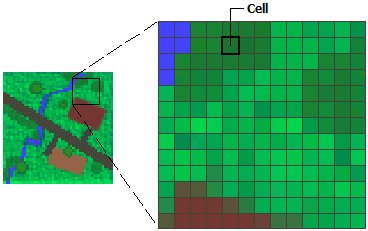
\includegraphics[width=0.75\columnwidth]{img/rasterdaten}\\
	\caption[]{Rasterdaten. Quelle ArcGis Dokumentation\footnotemark}
	\label{img:rasterdaten}
\end{figure}
\footnotetext{\footnote{\url{http://help.arcgis.com/de/arcgisdesktop/10.0/help/index.html#/na/009t00000002000000/}}}

\subsubsection{GeoTIFF}
TIFF(.tiff) ist ein Bildformat, welches Rasterdaten verlustfrei speichert. GeoTIFF erweitert dieses Format um Metadaten, wie der Projektion und den Geo-Koordinaten des Bildausschnittes. Diese Eigenschaften machen das Format attraktiv für die Speicherung großer Gebietskarten. Diese könne in Abhängigkeit zum erfassten Gebiet und dessen Auflösung mehrere Gigabyte umfassen. \\
Für die Darstellung von großen Rasterdaten, insbesondere in einer Client \& Server Architektur sind GeoTIFF Dateien daher ungeeignet und werden zu diesem Zweck in eine Mercator Pyramide (siehe \ref{sub:MercatorPyramide}) umgewandelt.


\subsection{Quadtree}
Quadtrees\cite{QuadTrees} sind ein Referenzierungsmodell, zur Aufteilung von zweidimensionalen Flächen in einer Baumstruktur. Jede Fläche wird in genau vier Unterbereiche (Kindknoten) unterteilt. Dies geschieht rekursiv bis zur gewünschten Tiefe. Diese Form der Flächenaufteilung wird u.a. für Mercator Pyramiden (siehe \ref{sub:MercatorPyramide}) verwendet.


\subsection{Mercator Pyramide}
\label{sub:MercatorPyramide}
Raster Pyramiden bestehen aus gleichgroßen Teilabschnitten einer größeren Rasterdatei in der Mercator Projektion, bei der jede Ebene eine Detailstufe (Zoomstufe) bildet. Sie sind eine Implementation der Quadtrees. \par
Die Mercator Projektion ist die Abbildung der Erdoberfläche auf eine quadratische Fläche. Für jede Detailstufe werden quadratische Kacheln gleicher Größe generiert. \\
Beginnend mit einer Kachel auf Detailstufe 0 vervierfachen sich die Anzahl der Kacheln auf jeder Ebene, bis zur gewünschten Tiefe. Die Verzweigung entspricht einem Quad-Tree, also einem Baum mit jeweils vier Kindelementen. Üblich sind Kachelgrößen von 256x256 Pixel, 19 Stufen und das Dateiformat .png. \\
Dieses Verfahren erlaubt es, dem Benutzer einer Webanwendung beliebig große Dateien ohne sichtbaren Qualitätsverlust zu präsentieren.\\
\begin{figure}[H]
	\centering
	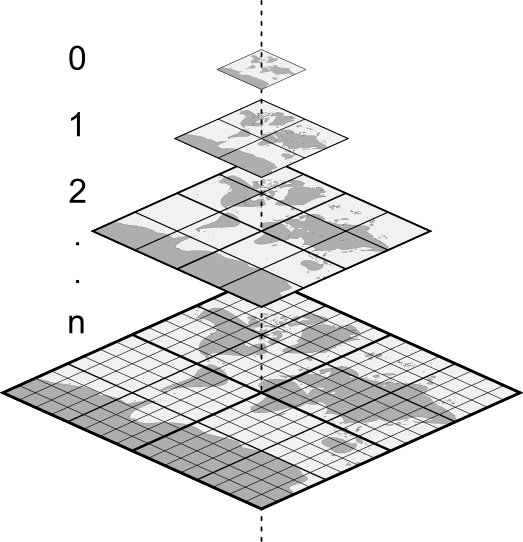
\includegraphics[width=0.6\columnwidth]{img/mercator_pyramid.png}\\
	\caption[]{Mercator Kachel Pyramide}
	\label{img:mercator_pyramid}
\end{figure}


\subsection{Quadkeys}
\label{Quadyeys}
Die Bing Quadkeys benennen die Flächen einer Mercator Pyramide mit einem Wert. Gewöhnlich werden Mercator Pyramiden mit Z/X/Y bezeichnet, wobei Z die Detailstufe, X die X-Achse und Y die Y-Achse ausmachen.\\
Quadkeys codieren die Position der Fläche, indem für jede Detailstufe eine Ziffer zwischen 0 und 3 hinzugefügt wird. Siehe hierfür Abb. \ref{img:bing_quads}.\\
\begin{figure}[H]
	\centering
	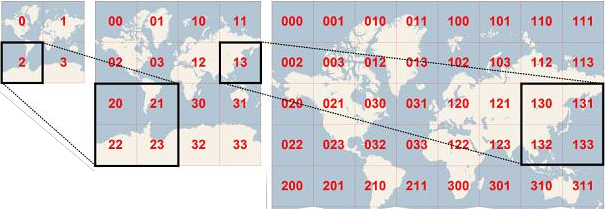
\includegraphics[width=1\columnwidth]{img/bing_quads.png}\\
	\caption[]{Bing Quadkeys\cite{BingQuadkeys}}
	\label{img:bing_quads}
\end{figure}



\section{Grundprojekt}
Der Begriff Geoinformationssystem(GIS) umfasst die Speicherung, Manipulation, Organisation und Darstellung von räumliche Daten. Diese Daten werden im MARS Framework als Basis für Agentensimulationen genutzt.\\
MARS DEIMOS stellt diese Daten dar und ermöglicht es dem Benutzer Daten für Simulationen auszuwählen. Um eine bessere Benutzbarkeit zu erreichen sollen die Daten auf Korrektheit geprüft werden.\\
Eine unmittelbare Korrektur der erkannten Fehler soll nur in geringem Maße durchgeführt werden. Grund hierfür ist die Existenz von bekannten und etablierten GIS-Werkzeugen wie ArcGIS, QGIS und GRASS, die für derartige Aufgaben konzipiert wurden.\par
Voraussetzung für ein zukunftssicheres Design sind, stabile und dokumentierte Softwarelösungen für die Analyse und Manipulation, sowie eine dauerhafte Speicherung der GEO-Daten.\\
Ziel des Grundprojektes ist es, die aktuelle Situation zu dokumentieren und Verbesserungsvorschläge zu erarbeiten.


\subsection{Technologievergleich}
Für die Verarbeitung von Geodaten gibt es zahlreiche Bibliotheken mit unterschiedlichen Einsatzgebieten. Folgende kommen für die Analyse und Manipulation von GIS-Daten in Betracht.

\subsubsection{Geospatial Data Abstraction Library (GDAL) [C/C++]}
GDAL ist eine, in C/C++ geschriebene Geo-Bibliothek für Raster und Vektordaten. Es wird in vielen Werkzeugen als Grundlage verwendet. Werkzeuge, die GDAL verwenden sind u.a. ArcGIS, QGIS, GRASS, Google Earth, die Programmiersprache \enquote{R}, sowie die im folgenden genannten Werkzeuge mit Außnahme GeoTools und dem GeoServer.\\
GDAL über den Aufruf der Konsolenanwendung direkt zu nutzen ist möglich, jedoch nicht zu empfehlen. Insbesondere die Auswertung von Rückgabewerten ist mit der unmittelbaren Verwendung umständlich, da die Konsolenausgaben interpretiert werden müssen.\\
Abhilfe können eine Vielzahl von GDAL Wrapper Bibliotheken schaffen. Diese ermöglichen eine bessere Handhabung.

\subsubsection{SharpMap [C\#]}
SharpMap ist ein Geospatiale Bibliothek für C\#, welche bereits in MARS LIVE verwendet wird. SharpMap unterstützt verschiedene Vektorformate, darunter Shapefiles. Die Unterstützung von Rasterdaten geschieht durch GDAL. Für die Darstellung von Kartendaten kann der Web Map Service (WMS) der The Open Source Geospatial Foundation (OSGeo) verwendet werden.\\
Die Dokumentation von SharpMap beschränkt sich auf 5 kurze Anwendungsbeispiele, eine komplette Klassendokumentation ist nicht vorhanden.
	
\subsubsection{DotSpatial [C\#]}
DotSpatial ist neben SharpMap eine weitere Möglichkeit Geospatiale Operation auf Geodaten in C\# durchzuführen. Im Vergleich zu SharpMap stehen dem Entwickler neben Tutorials und Code Ausschnitten auch ein Getting started Guide und eine SDK Dokumentation einiger Komponenten zur Verfügung.
	
\subsubsection{GeoTools [Java]}
\label{GeoTools}
GeoTools unterscheidet sich von den bereits genannten Werkzeugen insofern, als dass es in Java geschrieben wurde, welches bis jetzt nicht Teil der Websuite ist. Java als Sprache wird in der MARS Arbeitsgruppe bis jetzt nur im ConfigService eingesetzt. Durch den Einsatz von Docker ist dies allerdings nicht als Problem anzusehen, da eine heterogen gestaltete Softwarearchitektur dem Microservices Ansatz entspricht.\\
Die Bibliothek basiert als einzige der genannten Lösungen nicht auf GDAL als Basis. GeoTools ist Teil der Open Source Geospatial Foundation (OSGeo).\\
Es verfügt neben einem Quickstart Guide und einer API Dokumentation, über einen User Guide und zahlreiche Programmbeispiele. Die Dokumentationen sind ausgesprochen ausführlich und sehr aktuell. Das Projekt ist aktueller als jedes der anderen genannten Bibliotheken.

\subsubsection{GeoServer}
\label{subsubsubsec:GeoServer}
Der GeoServer ist eine Verwaltungssoftware für Geodaten, basierend auf Java und PostGIS. Unterstützt werden eine Vielzahl von Raster-/ und Vektorformaten. Der GeoServer erlaubt neben der Verwaltung auch die Bearbeitung von Geodaten, sowie eine Darstellung mit Hilfe von OpenLayers. All diese Funktionalitäten lassen sich über eine Weboberfläche bedienen.\\
Mittels einer ausführlichen REST Schnittstelle lassen sich die Geoserver Abfragen in andere Anwendungen integrieren.

\subsubsection{GeoNode [Python]}
GeoNode ist keine Bibliothek, es handelt sich hierbei um ein Content Management System (CMS) für Geodaten, basierend auf dem Python Webframework Django.\\
Nach der Installation bietet GeoNode eine ansprechende Benutzeroberfläche, über die sich Raster-/ und Vektordaten importieren lassen. Auf Basis dieser Layer lassen sich Karten zusammenstellen.\\
GeoNode speichert die importierten Daten nicht direkt in eine Datenbank, sondern nutzt eine Instanz des GeoServers (siehe Abs. \ref{subsubsubsec:GeoServer}). Obwohl der GeoServer ein Vielzahl von Formaten unterstützt erlaubt GeoNode derzeit (v2.3), nur den Import von Esri Shapefiles und GeoTIFF Dateien.


\subsection{Ergebnis}
Im Grundprojekt wurde eine Anforderungsanalyse durchgeführt. Auf Basis der ermittelten Anforderung wurde entschieden, dass der GeoServer zukünftig wieder für die Verwaltung von Geodaten verwendet werden soll. Des weiteren wird für die Berechnungen von Geooperationen ein Microservice erstellt, der alle nötigen Geooperation durchführt.

\subsubsection{Datenspeicherung}
In der Vergangenheit wurde vom GeoServer Abstand genommen, Performance Messungen im Rahmen des Grundprojektes haben jedoch gezeigt, dass ein entsprechend optimierter Geoserver durchaus in der Lage ist große Mengen an Geodaten zu verwalten.\\
Getestet wurde die Importgeschwindigkeit mit jeweils einer kleinen und einer großen Esri Ascii(.asc) Datei und einem Shapefile(.shp). Die Kleinen Dateien haben, komprimiert in einer .zip Datei eine ungefähre Größe von 400kB und die großen Dateien eine Größe von 500MB.\\
Es ist zu beachten, dass die Importzeiten unter localhost durchgeführt wurden und Die Ergebnisse Mittelwerte sind.\\
\begin{table}[H]
	{\tabulinesep=2mm
	\begin{center}\begin{tabu}{ |c|r|r| }
		\hline
		& \textbf{Shapefile} & \textbf{.asc Datei} \\ \hline
		kleine Datei & 200 ms & 70 ms \\ \hline
		große Datei & 8.800 ms & 3.500 ms \\ \hline
	\end{tabu}\end{center}}
	\caption{GeoServer Import Performance}
\end{table}

\subsubsection{Datenverarbeitung}
Viele Arbeiten, wie die Konvertierung von Geodaten und die Generierung von Bilderpyramiden sind direkt über den GeoServer möglich.\\
Für die weiterführende Verarbeitung und die inhaltliche Validitätsprüfung wird eine zentrale Komponente geschaffen, die lose an die Websuite gekoppelt ist. Diese Komponente besteht aus einer erweiterbaren Bibliothek auf Basis von GeoTools (siehe \ref{GeoTools}).\\



\section{Hauptprojekt}
Ziel des Hauptprojektes ist es, die spatiale Eingrenzung für alle Geodaten zu ermöglichen und die reduzierten Datensätze zu persistieren.\\
Außerdem soll der GIS-Import für den GeoServer entwickelt werden.\\
Des weiteren wird der Quad Algorithmus von Busch\cite{JanBusch} in die Websuite eingebaut.

\subsection{Spatiale Eingrenzung}
Die Anforderungsanalyse im Grundprojekt hat ergeben, dass GeoTools für die Verarbeitung von GIS-Daten am besten geeignet ist. Im Hauptprojekt soll ein entsprechender Service erarbeitet werden, der die notwendigen Operationen durchführt.


\subsection{GIS-Import}
Der GIS-Import ist Teil des allgemeinen Imports (siehe \ref{sub:Import}). Er ist dafür zuständig, Raster- und Vektordaten im GeoServer und der darunterliegenden PostGIS Datenbank zu speichern.


\subsection{Quad Algorithmus}
Bei der Speicherung von Rasterdaten wird jeder Datensatz als einzelne Datei abgelegt und es wird für den schnellen Zugriff im Web eine Mercatur Pyramide (siehe \ref{sub:MercatorPyramide}) generiert.\\
In bestimmten Anwendungsfällen ist es notwendig, dass Teilbereiche einer Rasterkarte referenziert werden und für den schnellen Zugriff abgelegt werden. Ein Anwendungsfall hierfür ist, dem Benutzer auswählbare Bereiche zur Verfügung zu stellen, welche die Ausdehnung der Simulation definieren.\\
\indent Eine Möglichkeit ist, den gewünschten Ausschnitt aus dem Quellmaterial in höchster Auflösung heraus zu schneiden und eine neue Mercator Pyramide zu generieren. Dies hat allerdings redundante Datenhaltung zur Folge. Besser ist es, QuadTiles aus der vorhandenen Bilder Pyramide zu referenzieren.\par
Der sog. Quad Algorithmus\cite{JanBusch} berechnet auf Basis einer geometrischen Form (z.B. Shapefile oder GeoJSON) die minimale Menge an Quadtiles, die nötig sind, um die Fläche komplett darstellen zu können und dabei den minimalen Overhead zu erreichen. Siehe Abb. \ref{img:shape2quads}.\\
Die zu speichernden Daten beschränken sich bei diesem Verfahren, auf ein Array von Quadkeys (siehe \ref{Quadyeys}).

\begin{figure}[H]
	\centering
	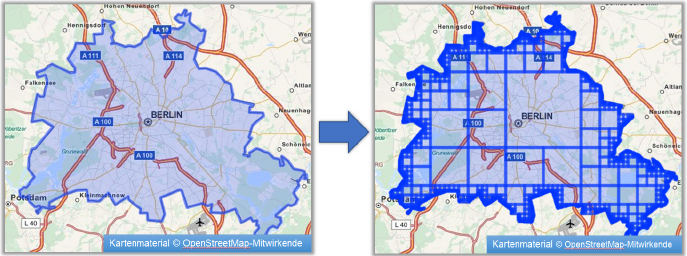
\includegraphics[width=1\columnwidth]{img/shape2quads.png} \\
	\caption[]{Umwandlung Shape in Quads am Beispiel Berlins. Quelle: \cite{JanBusch}}
	\label{img:shape2quads}
\end{figure}

Zur Reduktion des Rechenaufwandes wird zunächst die niedrigste Detailstufe errechnet, auf der die Berechnung begonnen werden kann. Hierzu wird von der obersten Ebene an, auf jeder Ebene überprüft, ob die gewählte Geometrie größer als ein Quadtile ist. Ist dies der Fall, so ist die aktuelle Ebene der Beginn des eigentlichen Algorithmus.\\
In parallelen Threads werden alle Tiles der aktuellen Ebene in drei Kategorien eingeteilt:
\begin{itemize}
	\item \textbf{Outside:} Quadtile liegt vollständig außerhalb
	\item \textbf{Within:} Quadtile liegt vollständig innerhalb
	\item \textbf{Intersects:} Quadtile liegt teilweise innerhalb / außerhalb
\end{itemize}
Tiles außerhalb des zu durchsuchenden Bereichs sind nicht teil der Ergebnismenge. Sie werden somit nicht weiter verarbeitet und die Rekursion wird abgebrochen.\\
Liegt ein Geometrisches Objekt vollständig in einer Kachel, so ist eine Tiefensuche ebenfalls nicht nötig. Das Tile wird der Ergebnismenge hinzugefügt.\\
Bei Kacheln der dritten Klasse, wird für die 4 tiefer gelegenen Kacheln jeweils in eigenen Threads rekursiv die gleiche Überprüfung durchgeführt.\\



\section{Masterarbeit - Spatialer Indikator}
Ökosysteme sind sehr komplexe Gebilde mit einer Vielzahl von Einflussfaktoren. Diese Konstrukte zu Verstehen ist die Voraussetzung dafür, Folgeabschätzungen durchführen zu können und somit, den stetig voranschreitenden Klimawandel zu begrenzen.\\
Spatiale Indikatoren können bei der räumlichen Analyse eingesetzt werden, um den klimatische Veränderungen besser zu verstehen (\cite{cline2014early} \cite{costa2014fragmentation} \cite{mattingly2014housing}).\par
Die Arbeitsgruppe um Hagenlocher et al. \cite{hagenlocher2014modeling} befasst sich mit den Ländern Westafrikas, da diese zu den am stärksten betroffenen, durch den Klimawandel gehören \cite{hamro2014livelihood}. Um besonders bedrohte Gebiete, sog. Hotspots zu extrahieren und diese Bereiche mit anderen vergleichbar zu machen wurde der spatial gemischte Indikator (SGI) entwickelt. Dieser stellt eine Weiterentwicklung des SI dar und wird mit Hilfe von arithmetischen Berechnungen aus verschiedenen homogenisierten Subindikatoren berechnet.\\

Der SGI gibt einen räumlich abhängigen Wert an, der geographische Gebiete in Bezug auf eine bestimmte Kennzahl vergleichbar macht \cite{anselin1995local}. Zur Berechnung des SGI müssen die Datensätze zunächst wert-normalisiert und anschließend segmentiert(regionalisiert) und klassifiziert werden. Abb. \ref{img:Spatialer_Indikator} zeigt den allgemeinen Ablauf.\\
\begin{figure}[H]
	\centering
	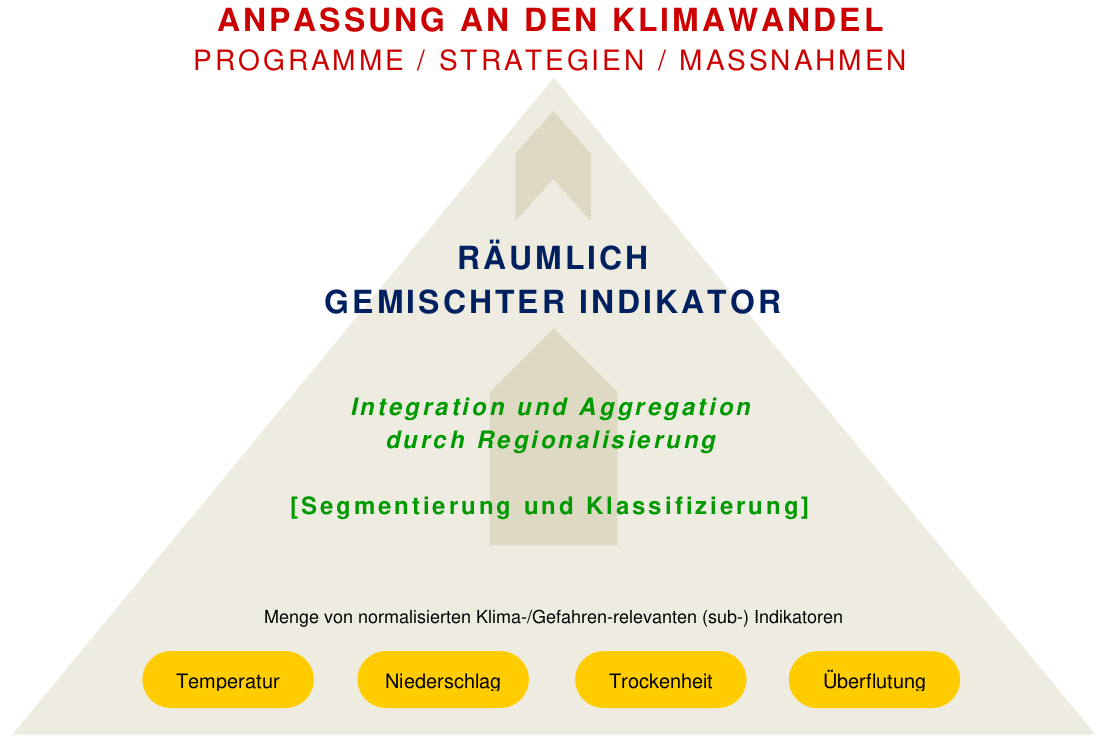
\includegraphics[width=1\columnwidth]{img/Spatialer_Indikator.png} \\
	\caption[]{Spatialer Indikator. Quelle: \cite{mariuszMaster}}
	\label{img:Spatialer_Indikator}
\end{figure}


\subsection{Voraussetzungen}
Für die Errechnung des SGI gelten bestimmt Prämissen, denen die Daten genügen müssen.\\
Der gemischte Indikator über ein Bereich wir aus verschiedenen Datensätzen errechnet. Eine korrekte Aussage kann nur getroffen werden, wenn die Daten den gleichen geographischen Bereich referenzieren.\\
Die Auflösung der Datensätze ist häufig unterschiedlich. Beispielsweise können Temperaturdaten stündlich aufgenommen sein und Niederschlagsdaten täglich. Eine entsprechende Inter- bzw. extrapolieren ist zwingend erforderlich.\\
Die einzelnen Daten müssen in GIS Formaten vorliegen. Hierbei handelt es sich um Formate, die neben den eigentlichen Daten Metadaten abspeichern können. Gängige Formate sind: *.shp, *.asc oder GeoJSON.\\
Die Layer, auf denen sich die Informationen befinden müssen georeferenziert sein, es muss also in den erwähnten Metadaten hinterlegt sein, für welchen Bereich und ggf. Zeitraum die Daten gültig sind.


\subsection{Vorbereitung}
 Es muss mittels GIS-Operationen eine gemeinsame Schnittmenge aus den, zur Verfügung stehenden Daten gebildet werden.\\
 Diese Fläche wird in verschiedene, gleichgroße Quadranten aufgeteilt um später eine gleich gewichtete Aussage zu erhalten. Die maximale Feingranularität der Quadranten hängt von der Auflösung der Daten ab, eine zu feine Unterteilung führt nicht zur Verbesserung des Ergebnis, jedoch zu höherem Rechenaufwand.\\
 Die Werte, der einzelnen Eingabeparameter müssen Wert-normalisiert werden. Üblich ist die Bildung des SGI über Farbwerte eins Graustufenbildes. Eine Normalisierung von 0 bis 255 ist hier der Regelfall. Abbildung \ref{img:Wertnormalisierung} zeigt die Formel zur Normalisierung.\\
 \begin{figure}[H]
 	\centering
 	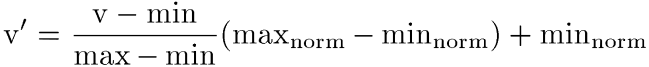
\includegraphics[width=1\columnwidth]{img/min_max_normalize.png} \\
 	\caption[]{Wertnormalisierung. Quelle: \cite{hagenlocher2014modeling}}
 	\label{img:Wertnormalisierung}
 \end{figure}
 
 In Abhängig der Eingabewerte zueinander, ist es gegebenenfalls notwendig eine Gewichtung einfließen zu lassen. Diese ist Domain abhängig und kann nicht generell festgelegt werden.\\
 Abschließend wird aus jedem Teilquadranten der SGI gebildet.\\


\subsection{Durchführung}
Die Bildung des SGI, mit den vorbereiteten Daten geschieht in drei Schritten: Segmentierung, Klassifizierung und Verschneidung.

\subsubsection{Segmentierung}
Nach Stepinski et al. \cite{stepinski2006automatic} werden bei der Segmentierung kleine Teile eines Bildes auf Basis von homogenen Eigenschaften unterteilt. Für die Durchführung wird das Verfahren der objekt-basierte Bildanalyse (OBIA) \cite{hay2006object} eingesetzt. Hierbei werden anhand von Farbwerten einzelne Objekte aus einem Bild herausgearbeitet, welche für die Klassifizierung verwendet werden.


\subsubsection{Klassifizierung}
Bei der Klassifizierung werden Grundinformationen der einzelnen Bereiche entfernt, um die Unterschiede von Bereichen besser heraus arbeiten zu können und Muster zu erkennen. Anhand von domainspezifischen Regeln werden Informationen herausgearbeitet.\\
Es kommen entsprechend des gewünschten Ergebnis andere Algorithmen zum Einsatz. Gängig sind die Klassifizierung durch Bestimmung der Häufigkeiten oder Durchschnittswerte der Farbwerte.


\subsubsection{Verschneidung}
Bei der Verschneidung wird aus den einzelnen Subindikatoren der Segmentierung und Klassifizierung, der SGI für einen Bereich errechnet. Hagenlocher et al. \cite{hagenlocher2014modeling} nutzt hierfür den Cumulative climate change impact (siehe Abb. \ref{img:CCI_Formel}).
\begin{figure}[H]
	\centering
	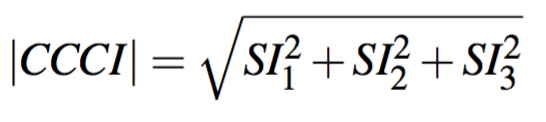
\includegraphics[width=0.5\columnwidth]{img/CCI_Formel.png} \\
	\caption[]{CCI Formel. Quelle: \cite{hagenlocher2014modeling}}
	\label{img:CCI_Formel}
\end{figure}

Die Verschneidung von Rasterdaten erfolgt über die Normalisierung verschiedener Zellen. Hierbei wird, ähnlich wie beim Downsampling von Bildern in eine geringere Auflösung, jeweils der, am häufigsten vorkommende Wert benachbarter Zellen genommen.\\
Dieser Wert wird klassifiziert und auf dessen Ergebnis wird die, oben genannten CCI Formel angewendet. Abb. \ref{img:CCIVerschneidung} zeigt diesen Ablauf. \\

\begin{figure}[H]
	\centering
	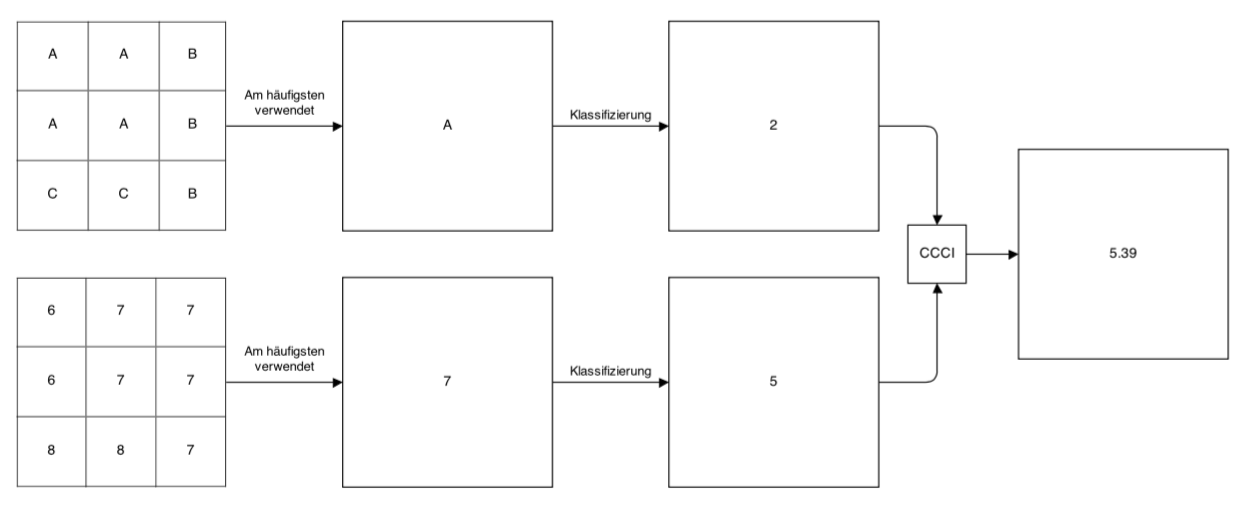
\includegraphics[width=1\columnwidth]{img/CCI_Verschneidung.png} \\
	\caption[]{CCI Verschneidung. Quelle: \cite{mariuszMaster}}
	\label{img:CCIVerschneidung}
\end{figure}

\subsubsection{Ergebnis}
Mit dem oben beschriebenen Verfahren hat die Arbeitsgruppe um Hagenlocher \cite{hagenlocher2014modeling} eine Karte zur Visualisierung von Klimarisiken in West-Afrika erstellt.\\
Die SGIs der einzelnen Bereiche wurden entsprechend ihrer Werte zwischen 0=weiß über gelb als Zwischenwert bis 1=rot dargestellt.\\
Zusätzlich wurde an den roten Hotspots die Art der Gefährdung in einem Tortendiagramm dargestellt. Siehe Abb. \ref{img:Klimahotspots}. \\

\begin{figure}[H]
	\centering
	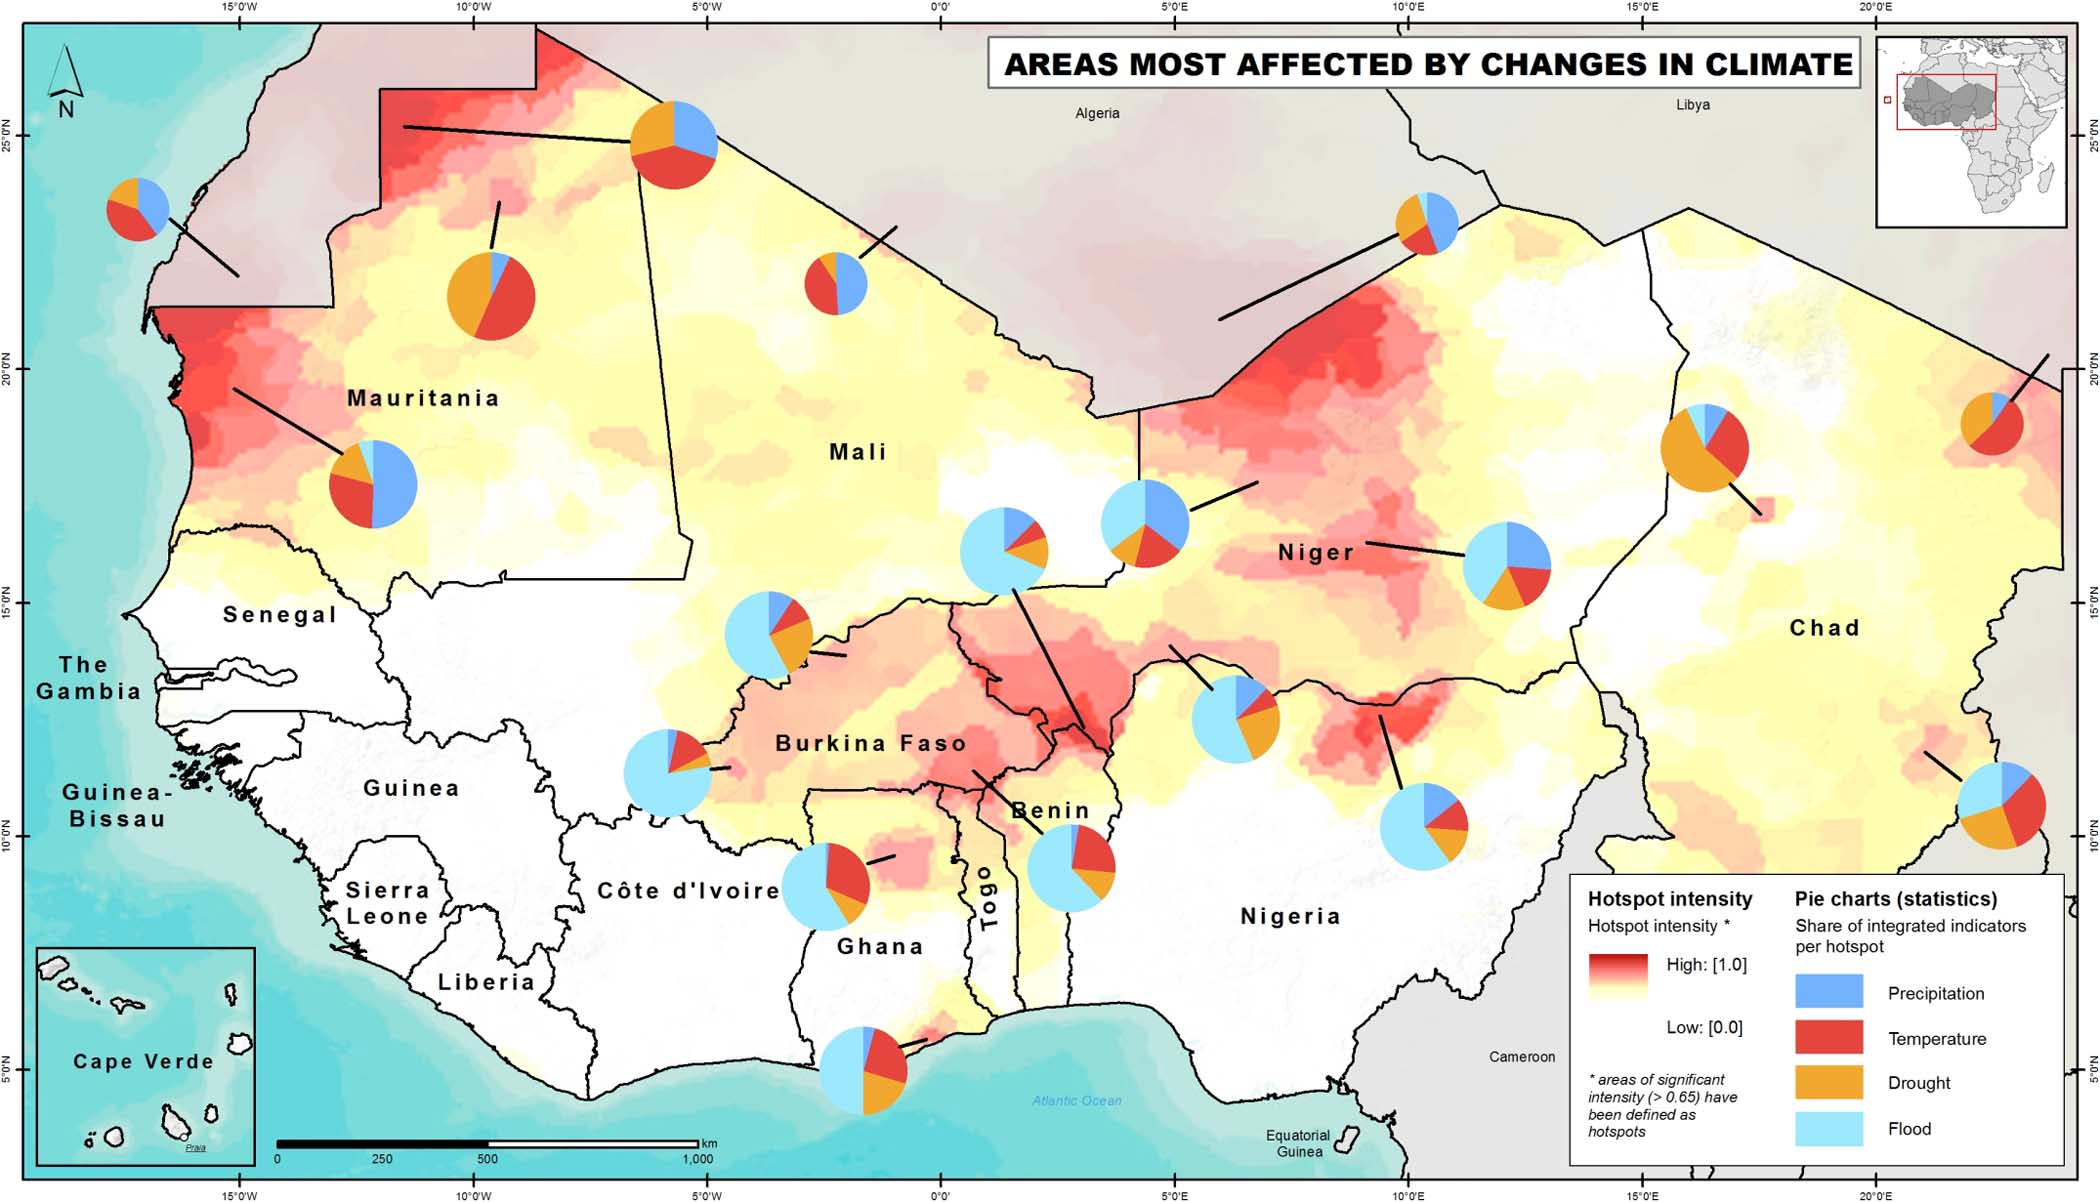
\includegraphics[width=1\columnwidth]{img/climate_hotspots.png} \\
	\caption[]{Klimahotspots. Quelle: \cite{hagenlocher2014modeling}}
	\label{img:Klimahotspots}
\end{figure}



\section{Zusammenfassung}
In dieser Arbeit wurde der aktuelle Stand zur Forschung an webbasierte GIS Datenverarbeitung beschrieben.\\
Im Grundprojekt wurden die technischen Grundlagen erarbeitet und Designentscheidungen getroffen, welche für die zukünftige Arbeit als Grundlage dienen soll.\\
Das Hauptprojekt befasst sich mit der spatialen Problematik, insbesondere der Handhabung von räumlicher Eingrenzung unterschiedlich gearteter Formen. Hierzu ist der Quad Algorithmus ein Vielversprechendes Werkzeug.\\
Das Kapitel zur Masterarbeit behandelt den SGI, welcher eine Methode zur Evaluierung von klimatischen Ereignissen darstellt.



\section{Ausblick}
Das Grundprojekt ist nahezu abgeschlossen, an dessen Themen werden daher keine großen Veränderungen mehr vorgenommen. \\
Die Themen des Hauptprojektes und der Masterarbeit stehen noch nicht endgültig fest. Im speziellen das Thema der Masterarbeit erfordert weitergehende Recherche, bei der die wissenschaftliche Relevanz für die Informatik zu prüfen ist.


\bibliographystyle{IEEEtran}
\bibliography{bibtemplate}

\end{document}
